\section{Генерирование реализаций случайных процессов}
Теперь посмотрим, как симулировать различные процессы. Начнём с самого 
простого~--- с пуассоновского потока.
\subsection{Генерирование пуассоновских случайных процессов}
\subsubsection{Однородный пуассоновский поток событий}
Для тех, кто забыл~--- определение пуассоновского потока дано в 
\hyperref[counting-process]{примере \ref*{counting-process}}. Единственная 
сложность в генерации реализации состоит в том, что нужно уметь генерирвать 
случайные величины из экспоненциального распределения. Но мы можем свободно 
генерировать случайные величины из \(\mathrm{U}(0, 1)\). Как получить из него 
экспоненциальное распределение? Для этого докажем одно утверждение:
\begin{lemma}[Метод обратного преобразования]
	Пусть \(X\)~--- случайная величина с неубывающей функцией распределения \(F 
	: \R \mapsto [0, 1]\). Введём обратную функцию \(F^{-1} : [0, 1] \mapsto 
	\R\) следующим образом: \(F^{-1}(u) = \inf\{x \in \R: F(x) \geq u\}\). 
	Тогда, если \(U \sim \mathrm{U}(0, 1)\), то \(F^{-1}(U)\) имеет функцию 
	распределения \(F\).
\end{lemma}
\begin{proof}
	Действительно, \(\Pr{F^{-1}(U) \leq x} = \Pr{U \leq F(x)} = F(x)\).
\end{proof}

Теперь покажем, как генерировать случайные величины из распределения 
\(\mathrm{Exp}(\lambda)\). Рассмотрим функцию распределения:
\[
	F(x) = 1 - e^{-\lambda x} \implies x = -\frac{1}{\lambda}\ln(1 - F(x)) 
	\implies F^{-1}(x) = -\frac{1}{\lambda}\ln(1 - x).
\]

Тогда по методу обратного преобразования \(-\ln(1 - U)/\lambda\) будет иметь 
распределение \(\mathrm{Exp}(\lambda)\). Теперь заметим, что \(1 - U \eqdist 
U\). Тогда получаем, что \(-\frac{1}{\lambda}\ln{U}\) будет иметь нужное 
распределение.

Теперь несложно написать алгоритм генерации реализации однородного 
пуассоновского потока.

\begin{algorithm}[H]
	\caption{Алгоритм генерации реализации однородного пуассоновского потока}
	\label{algo:homogenous-poisson}
	\begin{algorithmic}[1]
		\Require Интенсивность \(\lambda\), максимальное время \(T\).
		%\Ensure Реализация процесса.
		\State \(t \gets 0, I \gets 0, S \gets \emptyset\)
		\State сгенерировать \(U \sim \mathrm{U}(0, 1)\)
		\State \(t \gets t - \ln(U)/\lambda\)
		\algstore{homogenous-poisson}
	\end{algorithmic}
\end{algorithm}
\begin{algorithm}
	\begin{algorithmic}[1]
		\algrestore{homogenous-poisson}
		\While{\(t \leq T\)}
			\State \(I \gets I + 1, S(I) \gets t\)
			\State сгенерировать \(U \sim \mathrm{U}(0, 1)\)
			\State \(t \gets t - \ln(U)/\lambda\)
		\EndWhile
	\end{algorithmic}
\end{algorithm}

\begin{figure}[H]
	\centering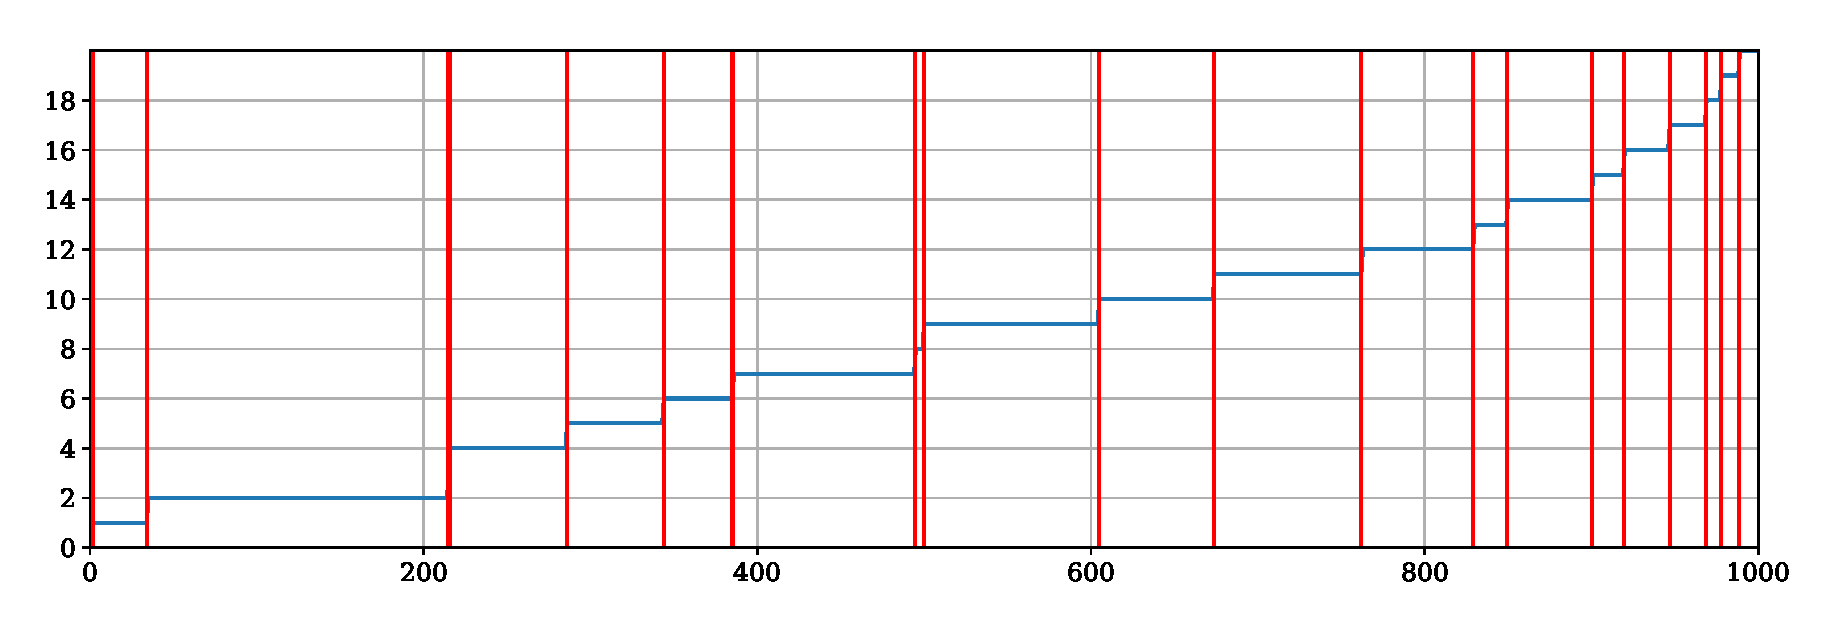
\includegraphics[width=\textwidth]{homogenous-poisson}
	\caption{Пример реализации пуассоновского потока с параметрами \(T = 
	1000\), \(\lambda = 0.02\)}
\end{figure}

\subsubsection{Неднородный пуассоновский поток событий}
Ранее мы смотрели на однородный пуассоновский процесс. Однородный он по той 
простой причине, что его интенсивность постоянна. Теперь скажем, что 
\(\lambda\)~--- это какая-то функция от \(t\). В таком случае получим 
\emph{неоднородный пуассоновский поток}. Определяется он почти так же, как и  
\hyperref[poisson-process-def]{однородный}, только немного изменяется третье 
свойство:
\[
	X_{t} - X_{s} \sim \mathrm{Pois}\left(\int\limits_{s}^{t} \lambda(x)\diff 
	x\right). 
\]

Но считать интегралы не очень приятно. Можно ли обойтись без них? Можно. 
Рассмотрим однородный пуассоновский поток \(N_{t}\) с интенсивностью 
\(\lambda\). Пусть событие, появляющееся в момент времени \(t\) 
``засчитывается'' с некоторой вероятностью \(p(t)\), то есть
\[
	\Pr{N_t = N_{t - \epsilon} + 1} = p(t), \quad \Pr{N_t = N_{t - \epsilon}} = 
	1 - p(t)
\]
Оказывается, что \(N_{t}\)~--- неоднородный пуассоновский поток событий с 
интенсивностью \(\lambda(t) = \lambda p(t)\). Этот результат называется 
\emph{теоремой Льюиса-Шедлера}.% Надо бы доказать в приложениях.

Пусть \(\tilde{\lambda} = \max_{t \in [0, T]} \lambda(t)\). Тогда алгоритм 
будет выглядеть так:
\begin{algorithm}[H]
	\caption{Алгоритм генерации реализации неоднородного пуассоновского потока}
	\label{algo:inhomogenous-poisson}
	\begin{algorithmic}[1]
		\Require Интенсивность \(\lambda(t)\), максимальное время \(T\).
		%\Ensure Реализация процесса.
		\State \(t \gets 0, I \gets 0, S \gets \emptyset, \)
		\State сгенерировать \(U_{1} \sim \mathrm{U}(0, 1)\)
		\State \(t \gets t - \ln(U_{1})/\tilde{\lambda}\)
		\While{\(t \leq T\)}
			\State сгенерировать \(U_{2} \sim \mathrm{U}(0, 1)\)
			\If{\(U_{2} \leq \lambda(t)/\tilde{\lambda}\)}
				\State \(I \gets I + 1, S(I) \gets t\)
			\EndIf
			\State сгенерировать \(U_{1} \sim \mathrm{U}(0, 1)\)
			\State \(t \gets t - \ln(U_{1})/\tilde{\lambda}\)
		\EndWhile
	\end{algorithmic}
\end{algorithm}
\begin{figure}[H]
	\centering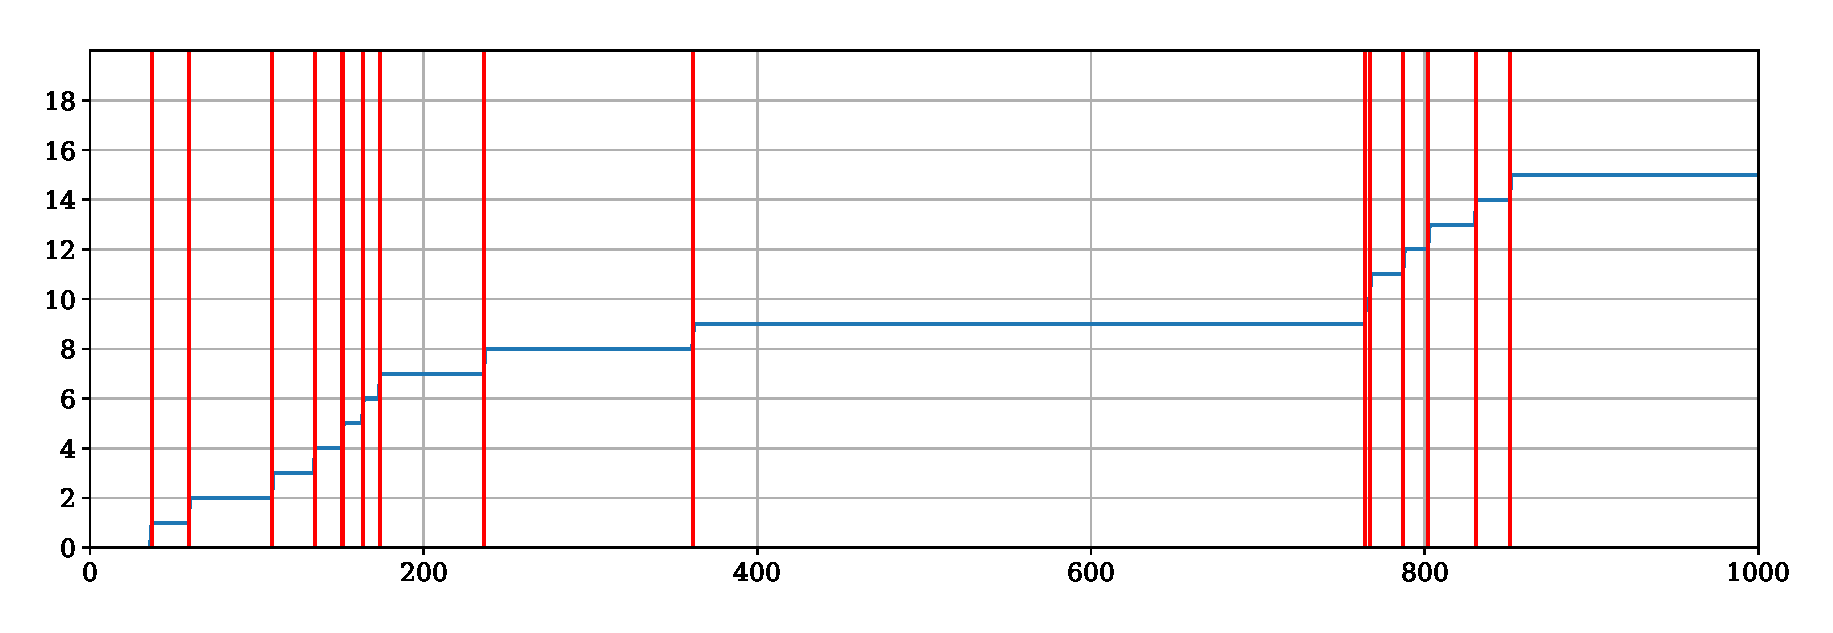
\includegraphics[width=\textwidth]{inhomogenous-poisson}
	\caption{Пример реализации неоднородного пуассоновского потока с 
	параметрами \(T = 1000\), \(\lambda(t) = (\sin(t/100) + 1)/100\).}
\end{figure}

\subsection{Метод стохастического интегрирования}
Как известно, дифференциальные уравнения описывают очень многое. Но, 
оказывается, их можно приспособить и для описания случайных процессов. Основное 
отличие состоит в том, что в данном случае функция, относительно которой 
решается уравнение, является случайной величиной. Такие дифференциальные 
уравнения называют \emph{стохастическими}.

Оказывается, что многие процессы, которые изучаются на практике, 
``управляются'' броуновским движением. Однако есть проблема: траектории 
винеровского процесса нигде не дифференцируемы почти наверное. Поэтому 
манипулирование с процессами такого типа потребовало создания собственного 
исчисления, называемого теорией \emph{стохастических интегралов}. Дадим 
определение:
\begin{definition}
	Пусть \(T = \{t_{k}\}_{k = 0}^{n}\)~--- некоторое 
	разбиение отрезка \([0, t]\). Далее, выберем точки \(\tau = \{\tau_{k}\}_{k 
	= 1}^{n}\) по правилу \(\tau_{k} \in [t_{k - 1}, t_{k}]\). Составим по 
	этому разбиению интегральную сумму:
	\[
		S_{n} = \sum_{k = 1}^{n} b(\tau_{k})(B_{t_{k}} - B_{t_{k - 1}})
	\]
	
	Стохастическим интегралом от неслучайной функции \(b(t)\) по броуновскому 
	движению \(B = (B_t)_{t \geq 0}\) называют предел интегральных сумм при 
	диаметре разбиения, стремящемся к нулю:\footnote{Вопрос о том, почему этот 
	предел вообще существует и каким образом последовательность частичных сумм 
	сходится к нему, оставим за кадром.}
	\[
		\int\limits_{0}^{t} b(x)\diff B_{x} = \lim_{\Delta T \to 0} S_{n}
	\]
\end{definition}
\begin{remark}
	Не стоит забывать, что \(B_{t_i} - B_{t_{i-1}} \sim \mathcal{N}(0, t_{i} - 
	t_{i - 1})\). Это поможет при симуляции процесса.
\end{remark} 

Многие стохастические процессы могут быть записаны в виде 
\[
	X_{t} = \int\limits_{0}^{t} a(x)\diff x + \int\limits_{0}^{t} b(x)\diff 
	B_{x},
\]
где \(a(x)\) и \(b(x)\)~--- некоторые неслучайные функции. Это же выражение 
можно записать в дифференциалах: \(\diff X_{t} = a(t)\diff t + b(t)\diff 
B_{t}\).

Как использовать этот метод? Примерно так же, как и в численном интегрировании: 
заменить дифференциал на малое изменение и суммировать.
\[
	X_{t + \epsilon} - X_{t} \approx a(t)\epsilon + b(t)(B_{t + \epsilon} - 
	B_{t}).
\]

\subsection{Метод гауссовских векторов}
Если нужно сгенерировать не слишком большую реализацию гауссовского процесса, 
то ситуация становится несколько проще. Как известно, у них все конечномерные 
функции распределения являются гауссовскими, поэтому реализация будет являться 
гауссовским вектором. Далее, нам известны математическое ожидание и 
ковариационная функция процесса. Из этого можно вытащить математическое 
ожидание и матрицу ковариаций нужного вектора.

Но есть проблема: как генерировать случайный гауссовский вектор с заданным 
распределением? Сходу это сделать не получится. Для этого проведём одно 
рассуждение.

Допустим, что вектор одномерный, то есть это просто случайная величина \(\xi 
\sim \mathcal{N}(\mu, \sigma^{2})\). Как из стандартного нормального 
распределения получить нужное распределение? Легко: \(\xi \eqdist \mu + 
\sigma\eta\), где \(\eta \sim \mathcal{N}(0, 1)\).

Оказывается, что для общего случая верно нечто похожее. Пусть \(\bm{\mu}\)~--- 
некоторый фиксированный вектор, \(\bm{\Sigma}\)~--- квадратная матрица, а 
\(\bm{\xi} \sim \mathcal{N}(\mathbf{0}, \mathbf{E})\). Какое распределение 
будет у случайного вектора \(\bm{\eta} = \bm{\mu} + \bm{\Sigma\xi}\)? Так как 
преобразование линейно, то это гауссовский вектор с параметрами
\begin{gather*}
	\E{\bm{\eta}} = \E{\bm{\mu} + \bm{\Sigma\xi}} = \E{\bm{\mu}} + 
	\bm{\Sigma}\E{\bm{\xi}} = \bm{\mu} \\
	\D{\bm{\eta}} = \E{\bm{\Sigma\xi}(\bm{\Sigma\xi})^{\intercal}} = 
	\bm{\Sigma}\E{\bm{\xi}\bm{\xi}^{\intercal}}\bm{\Sigma}^{\intercal} = 
	\bm{\Sigma}\bm{\Sigma}^{\intercal}.
\end{gather*}

Теперь вспомним один факт из линейной алгебры.
\begin{theorem}[Разложение Холецкого]
	Пусть \(\bm{\Sigma}\)~--- неотрицательно определённая симметричная матрица. 
	Тогда существует нижнетреугольная матрица \(\mathbf{C}\) с неотрицательными 
	членами на диагонали такая, что \(\bm{\Sigma} = \mathbf{CC}^{\intercal}\). 
	Если же \(\bm{\Sigma}\) положительно определена, то все члены 
	\(\mathbf{C}\) на диагонали строго положительны.
\end{theorem}

Выпишем формулы для вычисления матрицы \(\mathbf{C}\):
\[
	\mathbf{C}_{kk} = \sqrt{\bm{\Sigma}_{kk} - \sum_{j = 1}^{k - 1} 
	\mathbf{C}^{2}_{ki}}, \quad \mathbf{C}_{ij} = 
	\frac{1}{\mathbf{C}_{jj}}\left(\bm{\Sigma}_{ij} - \sum_{k = 1}^{j - 1} 
	\mathbf{C}_{ik}\mathbf{C}_{jk}\right)
\]

Отсюда понятно, как генерировать гауссовский вектор с заданным распределением 
\(\mathcal{N}(\bm{\mu}, \bm{\Sigma})\). Для этого мы независимо генерируем 
\(n\) случайных величин с распределением \(\mathcal{N}(0, 1)\) (это можно 
сделать с помощью того же преобразования Бокса-Мюллера) и получаем гауссовский 
вектор \(\bm{\xi}\). Далее, берём матрицу \(\mathbf{C}\) из разложения 
Холецкого и строим новый вектор \(\bm{\eta} = \bm{\mu} + \mathbf{C}\bm{\xi}\). 
Полученный вектор будет иметь нужное распределение.

\subsection{Генерирование гауссовских случайных процессов}
\subsubsection{Винеровский процесс}
Сначала разберёмся, как генерировать его с помощью гауссовских векторов. Для 
этого достаточно сгенерировать матрицу ковариаций и вектор матожиданий. Как 
известно, \(m(t) = 0\), а \(R(s, t) = \min(s, t)\).
\begin{figure}[H]
	\hspace{-0.01\textwidth} 
	\centering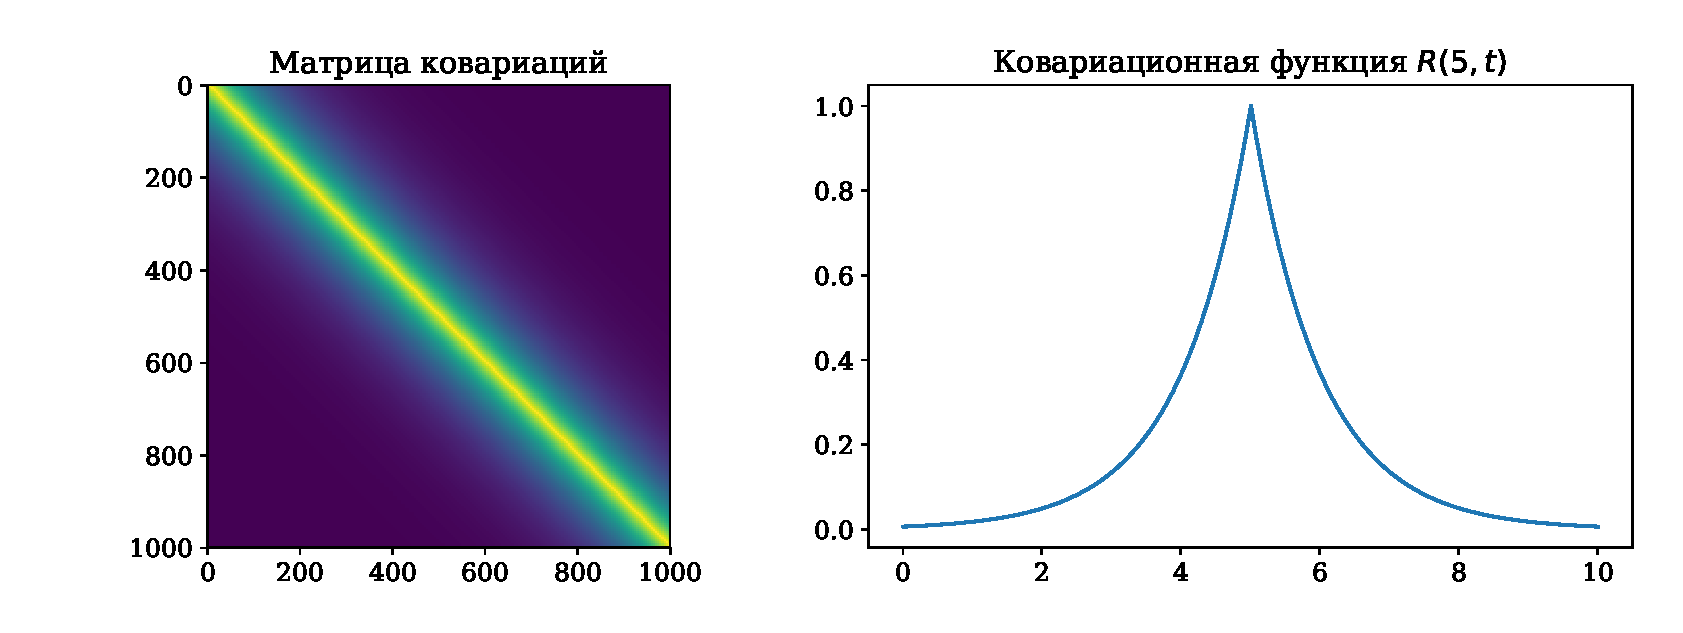
\includegraphics[width=\textwidth]{brownian-motion-covariation}
	\caption{Визуализация матрицы ковариаций и \(R(5, t)\) для \(t \in (0, 
	10)\).}
\end{figure}

Интереснее генерация с помощью стохастического интегрирования. Хотя и данном 
случае всё достаточно очевидно: \(B_{t}\) можно приблизить суммой достаточно 
большого числа номальных случайных величин:
\[
B_{t} = \int\limits_{0}^{t} \diff B_{x} \approx \sum_{k = 1}^{N} (B_{t_{k}} 
- B_{t_{k - 1}}).
\]

Для примера посмотрим на первые десять секунд. Для этого разобьём отрезок \([0, 
10]\) на 1000 равных кусков и посчитаем эту сумму. Это даст приемлемую точность.
\begin{figure}[H]
	\centering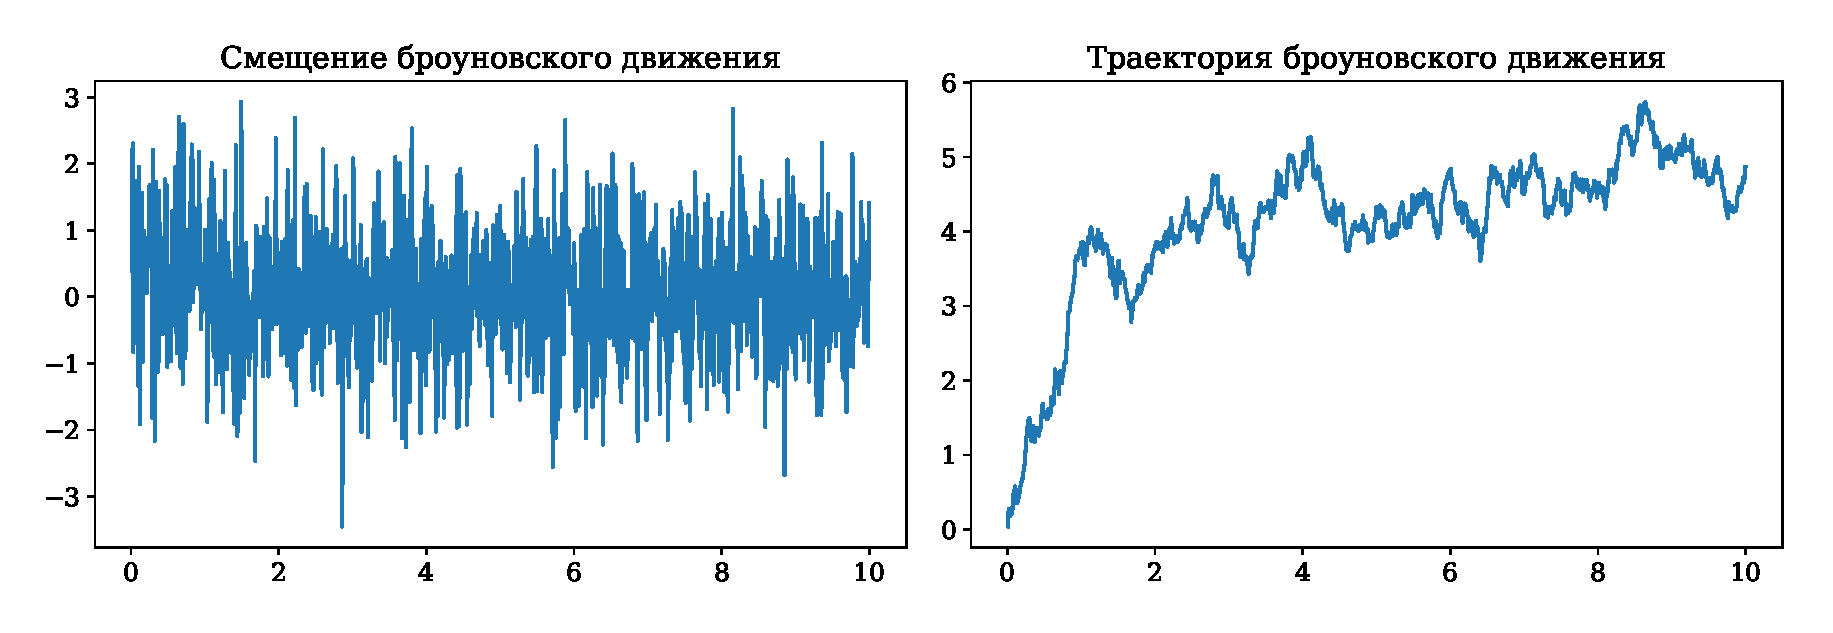
\includegraphics[width=\textwidth]{brownian-motion-integration}
	\caption{Пример реализации первых десяти секунд броуновского движения.}
\end{figure}

\subsubsection{Процесс Орнштейна-Уленбека}
\hyperref[ornstein-uhlenbeck-process]{Ранее} мы обсуждали процесс 
Орнштейна-Уленбека. Однако на самом деле он определяется немного по-другому:
\begin{definition}
	Случайный процесс \(X = (X_{t})_{t \geq 0}\), удовлетворяющий 
	стохастическому дифференциальному уравнению
	\[
	\diff X_{t} = \theta(\mu - X_{t})\diff t + \sigma \diff B_{t}, \quad 
	X_{0} = x_{0},
	\]
	называется процессом Орнштейна-Уленбека.
\end{definition}

Для того, чтобы получить ранее описанный процесс, нужно подставить \(\sigma = 
\sqrt{2}\), \(\theta = 1\), \(\mu = 0\) и \(x_{0} = 0\). Для генерации его 
реализации с помощью гауссовского вектора достаточно вспомнить, что \(\E{X_{t}} 
= 0\) и \(\cov(X_{t}, X_{s}) = e^{-|t - s|}\).

\begin{figure}[H]
	\hspace{-0.01\textwidth} 
	\centering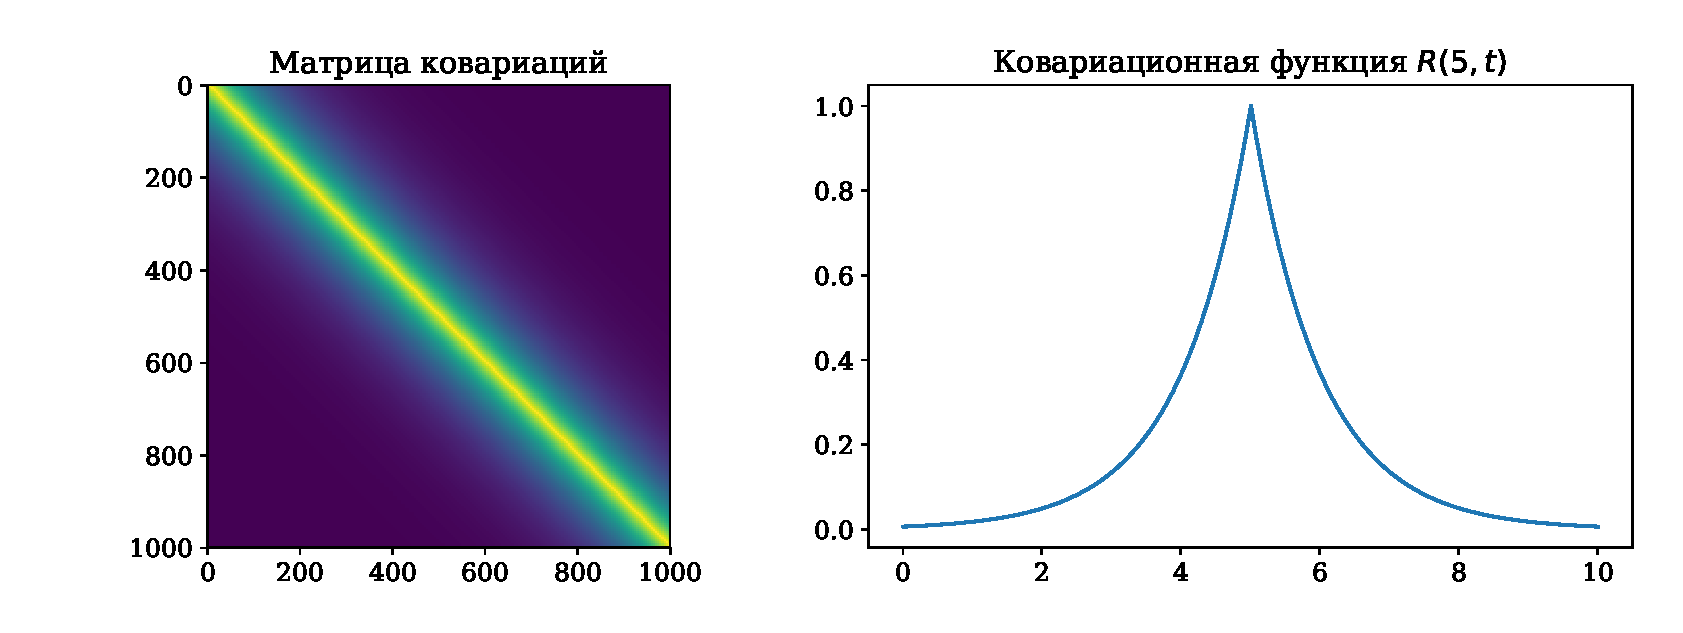
\includegraphics[width=\textwidth]{ornstein-uhlenbeck-covariation}
	\caption{Визуализация матрицы ковариаций и \(R(5, t)\) для \(t \in (0, 
		10)\).}
\end{figure}

Разностная схема устроена следующим образом:
\[
X_{t_{i + 1}} - X_{t_{i}} = \theta(\mu - X_{t_{i}})(t_{i + 1} - t_{i}) + 
\sigma(B_{t_{i + 1}} - B_{t_{i}}).
\]

\begin{figure}[H]
	\centering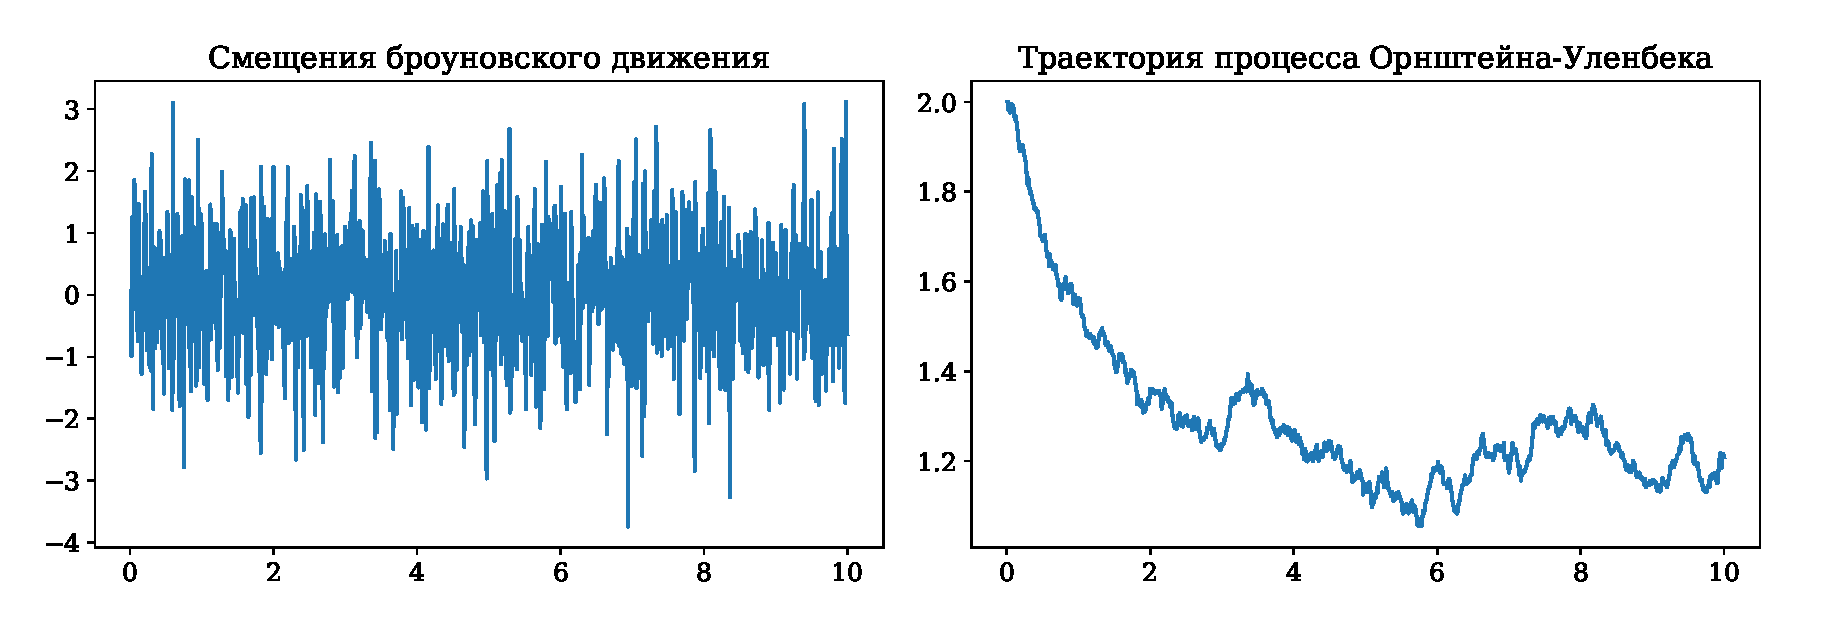
\includegraphics[width=\textwidth]{ornstein-uhlenbeck-integration}
	\caption{Пример реализации первых десяти секунд процесса Орнштейна-Уленбека 
		с параметрами \(x_{0} = 2\), \(\sigma = 0.1\), \(\mu = 1.2\), \(\theta 
		= 
		1\).}
\end{figure}

\subsubsection{Фрактальное броуновское движение}

Напоследок рассмотрим ещё один случайный процесс, называемый \emph{фрактальным 
броуновским движением}.
\begin{definition}
	Фрактальное броуновское движение с \emph{параметром Хёрста} \(H \in (0, 
	1)\)~--- это гауссовский случайный процесс с непрерывным временем 
	\(B^{H} = (B_{t}^{H})_{t \in [0, T]}\), удовлетворяющий следующим условиям:
	\begin{itemize}
		\item \(B^{H}_{0} = 0\) почти наверное,
		\item \(\E{B^{H}_{t}} = 0\) для всех \(t \in [0, T]\),
		\item \(\cov(B^{H}_{t}, B^{H}_{s}) = \frac{1}{2}(|t|^{2H} + |s|^{2H} - 
		|t - s|^{2H})\).
	\end{itemize}
\end{definition}

Оказывается, что если подставить \(H = 1/2\), то получится обычное броуновское 
движение.\footnote{Возникает вопрос о том, что делать с независимостью 
приращений. Но есть теорема, которая гласит, что фрактальное броуновское 
движение имеет независимые приращения только при \(H = 1/2\).} В остальных 
случаях получается некоторый гауссовский процесс. 
\begin{figure}[H]
	\hspace{-0.01\textwidth} 
	\centering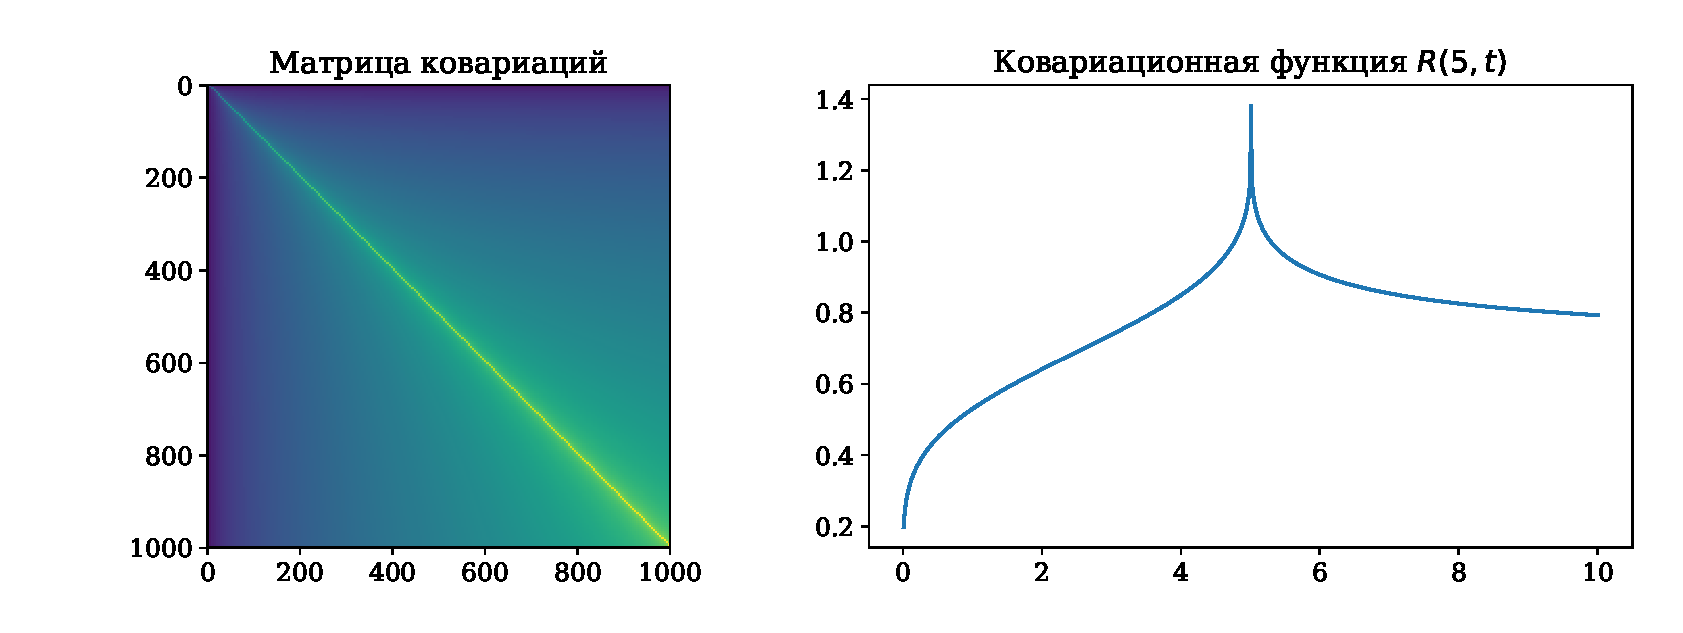
\includegraphics[width=\textwidth]{fractal-brownian-negative-covariation}
	\centering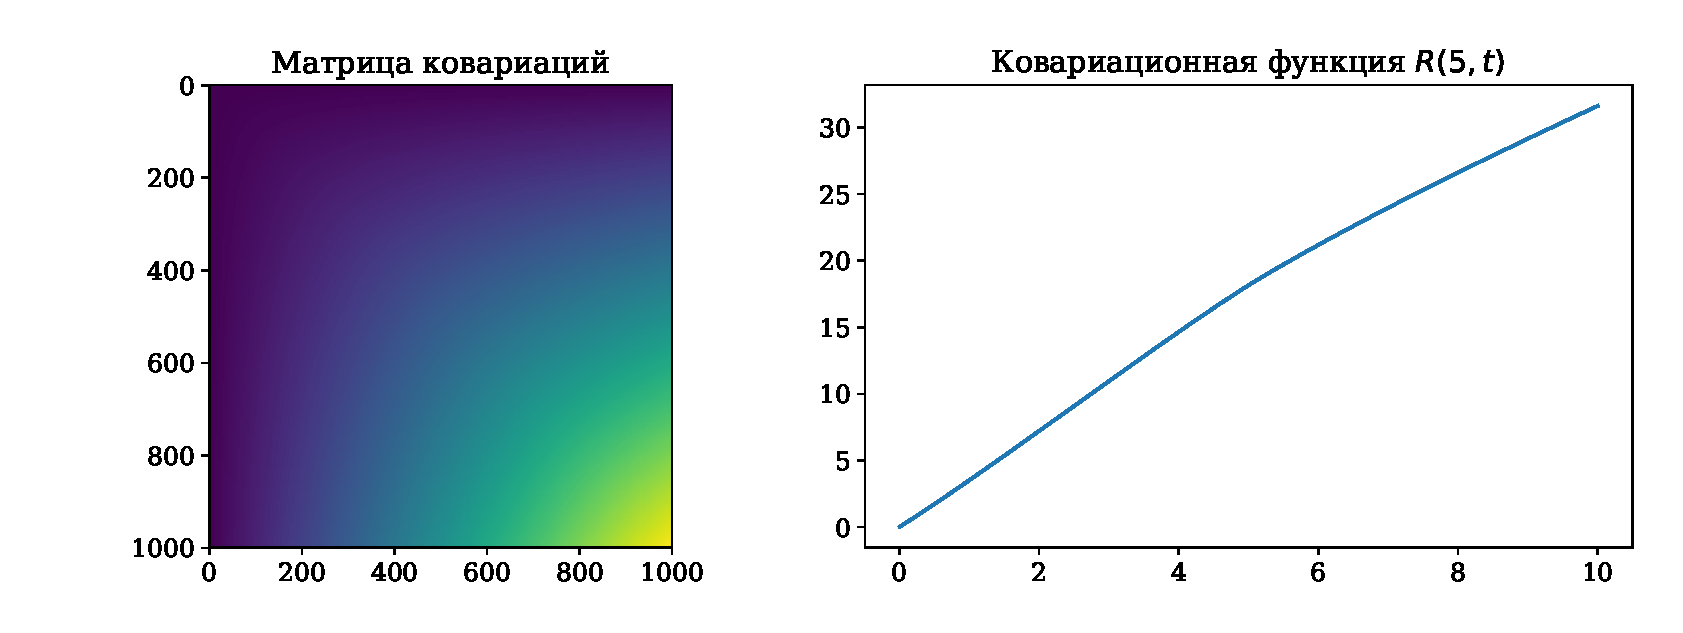
\includegraphics[width=\textwidth]{fractal-brownian-positive-covariation}
	\caption{Визуализация матрицы ковариаций и \(R(5, t)\) для \(t \in (0, 
		10)\) при \(H = 0.1\) и \(H = 0.9\).}
\end{figure}

После того, как была получена матрица ковариаций, дело остаётся за малым: 
получить нужнул реализацию с помощью разложения Холецкого. Я не буду описывать 
технические детали, ибо они и так очевидны. Теперь посмотрим, как себя ведут 
траектории в зависимости от параметра Хёрста.
\begin{figure}[H]
	\hspace{-0.01\textwidth} 
	\centering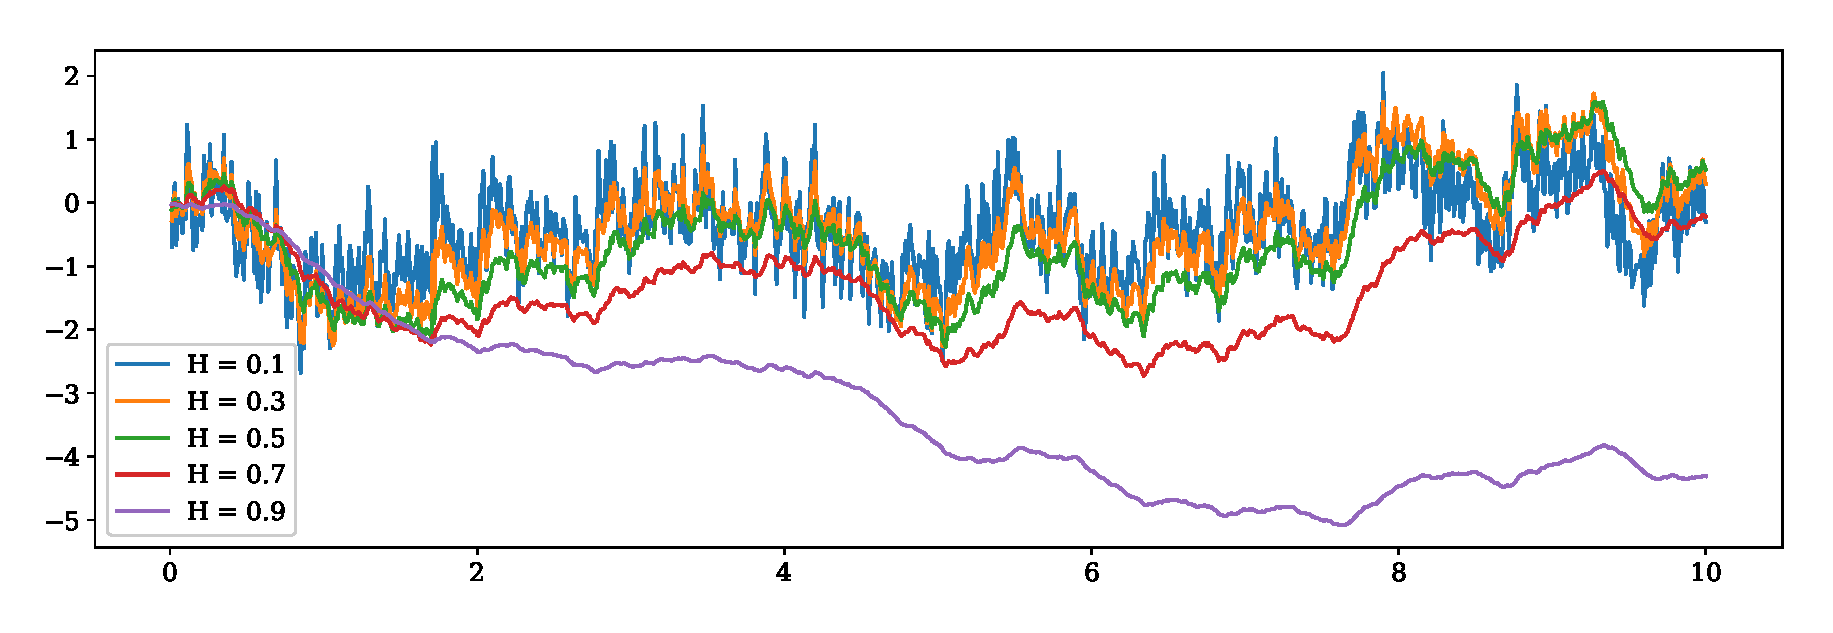
\includegraphics[width=\textwidth]{fractal-brownian-comparison}
	\caption{Пример реализаций первых десяти секунд фрактального броуновского 
	движения при разных параметрах Хёрста.}
\end{figure}

\section{Марковские цепи}
\subsection{Основные понятия}
Наверное, многие слышали про такое понятие, как марковские цепи. Что это такое? 
Перед этим дадим несколько необходимых понятий.

Пусть \(E\)~--- это некоторое дискретное (конечное или счётное) множество, 
которое называют \emph{пространством состояний}. Если система находится в 
состоянии \(i \in E\) в момент времени \(n\), то в момент времени \(n + 1\) она 
может перейти в состояние \(j \in E\) с \emph{переходной вероятностью} 
\(p_{ij}\). Это сразу даёт два свойства переходной вероятности:
\[
	\forall i, j \in E\ p_{ij} \geq 0 \text{ и } \forall i \in E\ \sum_{j \in 
	E} p_{ij} = 1.
\]
Переходные вероятности образуют \emph{матрицу переходных вероятностей} \(P = 
(p_{ij})_{i, j \in E}\). Теперь можно дать определение марковской цепи.
\begin{definition}
	\emph{Марковская цепь} с пространством состояний \(E\) и матрицей 
	переходных вероятностей \(P\)~--- это случайный процесс с дискретным 
	временем \(X = (X_{n})_{n \in \N}\), \(X_{n} \in E\), для которого
	\begin{itemize}
		\item известны начальные распределения \(\alpha_{i} \equiv \Pr{X_{0} = 
		i}\),
		\item верно \emph{марковское свойство}: для любого натурального \(n\) и 
		любых \(i_{0}, i_{1}, \dots, i_{n - 1}, i, j\)
		\[
		\Pr{X_{n + 1} = j \given X_{n} = i} = \Pr{X_{n + 1} = j \given X_{0} = 
			i_{0}, \dots, X_{n - 1} = i_{n - 1}, X_{n} = i} = p_{ij},
		\]
		если условные вероятности хорошо определены, то есть \(\Pr{X_{0} = 
		i_{0}, \dots, X_{n} = i} > 0\).
	\end{itemize}
\end{definition}
Неформально говоря, марковское свойство означает, что то, как система будет 
развиваться в текущий момент, не зависит от того, что было в прошлом и зависит 
только от настоящего.

Теперь вопрос: допустим, что у нас есть какая-то траектория (последовательность 
состояний). Какова её вероятность? Ответ на этот вопрос даст одна простая 
теорема.
\begin{theorem}[о состояниях марковской цепи]\label{markov-chain-states-theorem}
	Для любого натурального \(n\) и любых \(i_{0}, i_{1}, \dots, i_{n - 1}, i, 
	j\)
	\[
		\Pr{X_{0} = i_{0}, X_{1} = i_{1}, \dots, X_{n} = i_{n}} = 
		\alpha_{i_{0}} p_{i_{0}i_{1}} \ldots p_{i_{n - 1}i_{n}}.
	\]
\end{theorem}
\begin{proof}
	Индукция по количеству состояний. Пусть \(n = 0\). Тогда по определению 
	марковской цепи \(\Pr{X_{0} = i_{0}} = \alpha_{i_{0}}\).
	
	Теперь предположим, что утверждение верно для \(n\) состояний. Покажем, что 
	оно верно и для \(n + 1\) состояния. Действительно, по определению условной 
	вероятности и марковскому свойству
	\begin{multline*}
		\Pr{X_{0} = i_{0}, \dots, X_{n + 1} = i_{n + 1}} = \Pr{X_{0} = i_{0},  
		\dots, X_{n} = i_{n}}\Pr{X_{i + 1} = i_{n + 1} \given X_{n} = i_{n}} = 
		\\ = \alpha_{i_{0}} p_{i_{0}i_{1}} \ldots p_{i_{n - 1}i_{n}} 
		p_{i_{n}i_{n + 1}}. \qedhere
	\end{multline*}
\end{proof}
\begin{consequence}
	Для любого натурального \(n\) и любого \(i_{n} \in E\)
	\[
		\Pr{X_{n} = i_{n}} = \sum_{i_{0}, \ldots, i_{n - 1} \in E} 
		\alpha_{i_{0}} p_{i_{0}i_{1}} \ldots p_{i_{n - 1}i_{n}}.
	\]
\end{consequence}
\begin{proof}
	Прямое следствие из формулы полной вероятности и теоремы о состояниях 
	марковской цепи.
\end{proof}

Но обычно нас не интересует полный путь, а лишь начало и конец. Поэтому вводят 
вероятность перейти из состояния \(i\) в состояние \(j\) за \(n\) шагов:
\[
	p_{ij}^{(n)} = \Pr{X_{n} = j \given X_{0} = i}
\]

Чему равна эта вероятность? Воспользуемся теоремой о состояниях:
\begin{multline*}
	\Pr{X_{n} = j \given X_{0} = i} = \frac{\Pr{X_{n} = j, X_{0} = 
	i}}{\Pr{X_{0} = i}} = \\ = \sum_{i_{1}, \ldots, i_{n - 1} \in E} 
	\frac{\Pr{X_{0} = i, X_{1} = i_{1}, \dots, X_{n - 1} = i_{n - 1}, X_{n} - 
	j}}{\Pr{X_{0} = i}} = \sum_{i_{1}, \ldots, i_{n - 1} \in E} p_{ii_{1}} 
	\ldots p_{i_{n - 1}j}.
\end{multline*}

Если мы посмотрим на случай \(n = 2\), то полученное выражение очень похоже на 
скалярное произведение строк матрицы переходной вероятности. Оказывается, что 
это не так уж и далеко от истины.
\begin{theorem}
	Пусть \(P^{(n)} = (p_{ij}^{(n)})_{i,j \in E}\). Тогда \(P^{(n)} = P \cdot 
	P \cdot \ldots \cdot P = P^{n}\).
\end{theorem}
\begin{proof}
	Индукция по количеству шагов. База (\(n = 1\)) очевидна, так как 
	\(p_{ij}^{(1)} \equiv p_{ij}\). Теперь предположим, что утверждение 
	выполнено для \(n\) шагов. Тогда \(P^{(n)} = P^{n}\). Посмотрим на \(P^{(n 
	+ 1)}\):
	\begin{multline*}
		p_{ij}^{(n + 1)} = \Pr{X_{n + 1} = j \given X_{0} = i} = \sum_{i_{n} 
		\in E} \Pr{X_{n + 1} = j \given X_{n} = i_{n}, X_{0} = i}\Pr{X_{n + 1} 
		= i_{n} \given X_{0} = i} = \\ = \sum_{i_{n} \in E} \Pr{X_{n + 1} = j 
		\given X_{n} = i_{n}}\Pr{X_{n + 1} = i_{n} \given X_{0} = i} = 
		\sum_{i_{n} \in E} p_{ii_{n}}^{(n)}p_{i_{n}j}.
	\end{multline*}
	
	Отсюда получаем, что \(P^{(n + 1)} = P^{(n)}P = P^{n + 1}\).
\end{proof}

Однако это доказательство работает не всегда. Почему же? Потому что никто не 
обещал, что переходная вероятность не зависит от шага. Если она действительно 
не зависит, то говорят, что марковская цепь \emph{однородна}.

Теперь поговорим про состояния марковских цепей. В зависимости от переходных 
вероятностей поведение цепи в этом состоянии может кардинально различаться. 
Поэтому их классифицируют.

Первая классификация связана с важностью состояния. Может оказаться так, что из 
состояния можно выйти за конечное число шагов, но вернуться назад уже 
невозможно. Такие состояния не слишком влияют на долговременное поведение 
марковской цепи, поэтому их считают несущественными. Формализуем это:

\begin{definition}
	Пусть \(X = (X_{n})_{n \in \N}\)~--- марковская цепь с матрицей переходных 
	вероятностей \(P\) и дискретным множеством состояний \(E\). Будем называть 
	состояние \(i \in E\) \emph{несущественным}, если существует состояние 
	\(j\) и натуральное \(n\) такое, что \(p_{ij}^{(n)} > 0\), но \(\forall m 
	\in \N\ p_{ij}^{(m)} = 0\). В противном случае состояние называют 
	\emph{существенным}.
\end{definition}

Вторая классификация связана с возвращением. 
\begin{definition}
	Состояние \(i\) марковской цепи называется \emph{возвратным} (reccurent), 
	если 
	\[
		\Pr{X_{n} = i \text{ для бесконечно многих }n} = 1.
	\]
	Если же эта вероятность равна нулю, то состояние называют 
	\emph{невозвратным} (transient).
\end{definition}

\begin{wrapfigure}[13]{r}{0.5\textwidth}
	\begin{center}
		\begin{center}
			\begin{tikzpicture}
			\clip (-0.5,-0.5) rectangle (5.5,2.6);
			\Vertex[x=0,y=2]{A}
			\Vertex[x=3,y=2]{B}
			\Vertex[x=1.5,y=0]{C}
			\Vertex[x=5,y=2]{D}
			\Vertex[x=4,y=0]{E}
			\tikzstyle{LabelStyle}=[fill=white,sloped]
			\tikzstyle{EdgeStyle}=[post,bend left]
			\Edge(A)(B)
			\Edge(C)(A)
			\Edge(C)(B)
			\Edge(A)(C)
			\Edge(B)(C)
			\Edge(D)(E)
			\Edge(E)(D)
			\end{tikzpicture}
		\end{center}
	\end{center}
	\caption{Пример изображения марковской цепи в виде графа. В данном случае 
	\(E = \{A, B, C, D, E\}\). Отсутствие ребра означает, что переходная 
	вероятность равна нулю.}
\end{wrapfigure}

Так как на данный момент мы рассматриваем только дискретный случай, то у нас 
есть роскошь: можно смотреть на марковскую цепь, как на ориентированный граф, 
где вершины~--- это события, а вес ребра~--- переходная вероятность. Теперь 
вспомним, что в теории графов вводилось такое понятие, как связность. Для 
марковских цепей вводится похожее понятие.
\begin{definition}
	Состояние \(j\) марковской цепи называются \emph{достижимым} из состояния 
	\(i\), если существует такое натуральное \(n\), что \(p_{ij}^{(n)} > 0\). 
	Обозначение: \(i \to j\).
\end{definition}
\begin{definition}
	Существенные состояния \(i\) и \(j\) марковской цепи называются 
	\emph{сообщающимися}, если \(i \to j\) и \(j \to i\). Обозначение: \(i 
	\leftrightarrow j\).
\end{definition}

У этого понятия есть одно полезное свойство:
\begin{property}
	Сообщаемость задаёт отношение эквивалентности.
\end{property}
\begin{proof}
	Для начала нужно показать, что отношение сообщаемости рефлексивно. Пусть 
	\(i \in E\) существенно. Это означает, что существуют такие натуральные 
	\(m\) и \(n\), что \(p_{ij}^{(m)} > 0\) и \(p_{ji}^{(n)} > 0\). А это и 
	означает, что \(i \leftrightarrow i\).
	
	Коммутативность очевидна. Теперь покажем, что выполнена транзитивность. Для 
	этого достаточно показать, что если \(i \to j\) и \(j \to k\), то и \(i \to 
	k\). Действительно, если \(p_{ij}^{(m)} > 0\) и \(p_{jk}^{(n)} > 0\), то 
	\(p_{ik}^{(m + n)} \geq p_{ij}^{(m)}p_{jk}^{(n)} > 0\).
\end{proof}

В итоге мы получаем, что марковскую цепь можно разбить на классы сообщающихся 
вершин, коих будет не более, чем счётное число. Если такой класс один, то 
марковскую цепь называют \emph{неприводимой} (или \emph{неразложимой}).

Допустим, что мы разбили множество состояний марковской цепи на классы 
сообщаемости \(S_{1}, \dots, S_{n}, \dots\) и класс несущественных состояний 
\(S_{0}\). Как будет выглядеть матрица переходных вероятностей \(P^{(n)}\)? 
Оказывается, что она будет иметь блочный вид:
\[
	P^{(n)} = 
	\begin{pmatrix}
	S_{0} \to S_{0} & S_{0} \to S_{1} & S_{0} \to S_{2} & \ldots & S_{0} \to 
	S_{n} & \ldots \\
	0 & S_{1} \to S_{1} & 0 & \ldots & 0 & \ldots \\
	0 & 0 & S_{2} \to S_{2} & \ldots & 0 & \ldots \\
	\vdots & \vdots & \vdots & \ddots & \vdots & \ddots \\
	0 & 0 & 0 &\ldots & S_{n} \to S_{n} & \ldots \\
	\vdots & \vdots & \vdots & \ddots & \vdots & \ddots \\
	\end{pmatrix},
\]
где \(S_{i} \to S_{j}\)~--- блочная матрица переходных вероятностей из 
состояний класса \(S_{i}\) в состояния класса \(S_{j}\).

Последняя классификация вершин связана с возвращением в состояние. Введём 
понятие периода состояния.
\begin{definition}
	Пусть \(X = (X_{n})_{n \in \N}\)~--- однородная марковская цепь с матрицей 
	переходных вероятностей \(P\) и дискретным множеством состояний \(E\). 
	Число \(d_{i} = \gcd\{n \in \N \mid p_{ii}^{(n)} > 0\}\) будем называть 
	\emph{периодом} состояния \(j\). Если \(d_{j} > 1\), то состояние \(j\) 
	\emph{периодическое}, иначе же \(j\) \emph{апериодическое}.
\end{definition}

\begin{wrapfigure}[14]{r}{0.5\textwidth}
	\begin{center}
	\begin{tikzpicture}[scale=0.75,transform shape]
	\Vertex[x=2,y=0]{D}
	\Vertex[x=0,y=2]{B}
	\Vertex[x=4,y=2]{C}
	\Vertex[x=2,y=4]{A}
	\tikzstyle{VertexStyle}=[shape=coordinate]
	\Vertex[x=5,y=2]{F}
	\tikzstyle{LabelStyle}=[fill=white,sloped]
	\tikzstyle{EdgeStyle}=[post,bend right]
	\Edge[label=$0.5$](A)(B)
	\Edge(B)(D)
	\tikzstyle{EdgeStyle}=[post,bend left]
	\Edge[label=$0.5$](A)(C)
	\Edge(C)(D)
	\tikzstyle{EdgeStyle}=[relative=false,in=-90,out=-90]
	\Edge(D)(F)
	\tikzstyle{EdgeStyle}=[post,relative=false,in=90,out=90]
	\Edge(F)(A)
	\end{tikzpicture}
	\end{center}
	\caption{В данной марковской цепи периодическими будут состояния \(B\) и 
	\(C\).}
\end{wrapfigure}

Осталось ввести одно понятие, которое может понадобиться в дальнейшем. 
\begin{definition}
	Состояние \(i\) называется \emph{нулевым}, если \(p_{ii}^{(n)} \to 0\) при 
	\(n \to \infty\).
\end{definition}

Теперь посмотрим на какой-нибудь жизненный пример, который можно описать 
марковской цепью~--- например, простейшее случайное блуждание. Строится оно так 
же, как в \hyperref[random-walk]{примере \ref*{random-walk}}, только берётся 
распределение, принимающее значения 1, 0 и \(-1\) с какими-то вероятностями. 
Марковская цепь, симулирующая такой процесс, устроена просто. Множеством 
состояний является \(\Z\), а матрица переходных вероятностей задаётся так:
\[
	p_{ij} = \begin{cases}
	0, & |i - j| > 1 \\
	p_{0}, & j = i \\
	p_{1}, & j = i + 1 \\
	p_{2}, & j = i - 1 \\
	\end{cases}
\]

\begin{figure}[H]
	\begin{center}
		\begin{tikzpicture}
		\tikzset{node style/.style={state, circle}}
		\node[draw=none] (-3) {\(\cdots\)};
		\node[node style, right=of -3] (-2) {\(-2\)};
		\node[node style, right=of -2] (-1) {\(-1\)};
		\node[node style, right=of -1] (0) {\(0\)};
		\node[node style, right=of 0] (1) {\(1\)};
		\node[node style, right=of 1] (2) {\(2\)};
		\node[draw=none, right=of 2] (3) {\(\cdots\)};
		
		\draw[every loop,>=Stealth]
			(-3) edge[bend right=20,auto=right] node {} (-2)
			(-2) edge[bend right=20,auto=right] node {} (-3)
			(-2) edge[loop above] node {\(p_{0}\)} (-2)
			(-2) edge[bend right=20,auto=right] node {\(p_{1}\)} (-1)
			(-1) edge[bend right=20,auto=right] node {\(p_{2}\)} (-2)
			(-1) edge[loop above] node {\(p_{0}\)} (-1)
			(-1) edge[bend right=20,auto=right] node {\(p_{1}\)} (0)
			(0) edge[bend right=20,auto=right] node {\(p_{2}\)} (-1)
			(0) edge[loop above] node {\(p_{0}\)} (0)
			(0) edge[bend right=20,auto=right] node {\(p_{1}\)} (1)
			(1) edge[bend right=20,auto=right] node {\(p_{2}\)} (0)
			(1) edge[loop above] node {\(p_{0}\)} (1)
			(1) edge[bend right=20,auto=right] node {\(p_{1}\)} (2)
			(2) edge[bend right=20,auto=right] node {\(p_{2}\)} (1)
			(2) edge[loop above] node {\(p_{0}\)} (2)
			(2) edge[bend right=20,auto=right] node {} (3)
			(3) edge[bend right=20,auto=right] node {} (2);
		\end{tikzpicture}
	\end{center}
	\caption{Графическое изображение марковской цепи, соответствующей простому 
	случайному блужданию.}
\end{figure}
\begin{example}
	Пусть блуждание начинается в нуле и \(p_{0} = p_{1} = \nicefrac{1}{2}\). 
	Отсюда сразу же получаем, что \(p_{2} = 0\). Что мы можем сказать про такое 
	блуждание? А ничего хорошего. Все состояния несущественны, невозвратны и 
	нулевые.
\end{example}
\begin{example}
	Теперь изменим вероятности: \(p_{1} = p_{2} = \nicefrac{1}{2}\). Получится 
	так называемое \emph{симметричное случайное блуждание}. В таком случае мы 
	можем сказать, что нулевое состояние периодично с \(d_{0} = 2\), так как 
	есть ненулевая вероятность вернуться в начало за \(2k\) шагов (и понятно, 
	что вернуться за нечётное число шагов невозможно). Вообще, если и 
	\(p_{1}\), и \(p_{2}\) больше нуля, то все состояния существенны и 
	сообщаются.
\end{example}
\begin{example}
	Сузим множество состояний до \(\{-k, \ldots, -1, 0, 1, \ldots, k\}\) и 
	изменим вероятности перехода на границах: \(p_{kk} = p_{-k,-k} = 1\). 
	Получится \emph{случайное блуждание с поглощающими экранами}. В таком 
	случае существенными состояниями будут только \(\pm k\).
\end{example}

Вернёмся к возвратности. Как можно определить, является ли состояние 
возвратным? По определению это сдедать весьма непросто. Но есть теорема, 
которая упрощает жизнь.
\begin{theorem}
	Пусть \(f_{i} = \Pr{\exists\,n \in \N : X_{n} = i}\)~--- вероятность того, 
	что мы хотя бы раз попали в состояние \(i\). Тогда состояние \(i\) будет 
	возвратным тогда и только тогда, когда \(f_{i} = 1\).
\end{theorem}

Как посчитать \(f_{i}\)? Пусть \(A_{i}^{(n)} = \{\text{вернуться в }i\text{ 
ровно за }n\text{ шагов}\}\). Вероятность этого события равна:
\[
f_{i}(n) \equiv \Pr{A_{i}^{(n)}} = \Pr{X_{n} = i, X_{k} \neq i, k \in \{1, 
	\dots, n - 1\} \given X_{0} = i}
\]

Отсюда несложно получить, что \(f_{i}\) равна сумме \(f_{i}(n)\) по всем 
натуральным \(n\).
\begin{proof}
	Зафиксируем состояние \(i\). Пусть \(B_{k} = \{X_{n} = i \text{ хотя бы 
	}k\text{ раз}\}\). Это можно записать по-другому:
	\[
		B_{k} = \{\exists\,n_{1}, \ldots, n_{k} \in \N : X_{n_{1}} = i, \ldots, 
		X_{n_{k}} = i\}.
	\] 
	
	Что мы можем сказать про такие события? Во-первых, \(B_{k + 1} \subseteq 
	B_{k}\), так как если мы посетили состояние \(i\) \(k + 1\) раз, то мы его 
	посетили и \(k\) раз. Далее, марковское свойство даёт нам ``отсутствие 
	памяти''. Тогда \(\Pr{B_{k}} = f_{i}^{k}\). 
	
	Теперь заметим, что вероятность возвратности можно записать следующим 
	образом:
	\[
		\Pr{X_{n} = i \text{ для бесконечно многих }n} = \Pr{\bigcap_{n = 
		1}^{\infty} B_{n}}.
	\]
	
	По непрерывности вероятностной меры
	\[
		\Pr{\bigcap_{n = 1}^{\infty} B_{n}} = \lim\limits_{n \to \infty} 
		\Pr{B_{n}} = \lim\limits_{n \to \infty} f_{i}^{n} = 
		\begin{cases}
		1, & f_{i} = 1 \\
		0, & f_{i} < 1
		\end{cases} \qedhere
	\]
\end{proof}
\begin{theorem}\label{recurrent-condition-criterion}
	Пусть \(i\)~--- состояние марковской цепи. Оно будет возвратным тогда и 
	только тогда, когда расходится ряд \(\sum p_{ii}^{(n)}\).
\end{theorem}
\begin{proof}
	Зафиксируем состояние \(i\) и рассмотрим случайную величину
	\[
		V_{i} = \sum_{k = 1}^{\infty} \I\{X_{k} = i\} = \#\{n \in \N : X_{n} = 
		i\}.
	\]
	
	Что мы можем сказать про неё? Во-первых, \(\Pr{V_{i} \geq k} = \Pr{B_{k}} = 
	f_{i}^{k}\). Далее, мы можем посчитать матожидание двумя способами:
	\begin{gather}
		\E{V_{i}} = \E{\sum_{k = 1}^{\infty} \I\{X_{k} = i\}} = \sum_{k = 
		1}^{\infty} \Pr{X_{k} = i}  = \alpha_{i}\sum_{k = 1}^{\infty} 
		p_{ii}^{(n)}. \\
		\E{V_{i}} = \sum_{k = 1}^{\infty} k\Pr{V_{i} = k} = \sum_{k = 
		1}^{\infty} \left(\sum_{j = k}^{\infty} \Pr{V_{i} = j}\right) = \sum_{k 
		= 1}^{\infty} \Pr{V_{i} \geq k} = \sum_{k = 1}^{\infty} f_{i}^{k}.
	\end{gather}
	
	Теперь заметим одну вещь: если матожидание конечно, то вероятность того, 
	что \(V_{i} = +\infty\), нулевая. Тогда мы сразу получаем желаемое: если 
	\(i\) возвратно, то \(f_{i} = 1\) и ряд \(\sum p_{ii}^{(n)}\) расходится. 
	Иначе же ряд \(\sum f_{i}^{n}\) сходится и матожидание конечно. 
	Следовательно, ряд \(\sum p_{ii}^{(n)}\) сходится.
\end{proof}

Теперь применим эту теорему к простейшим случайным блужданиям.
\begin{theorem}
	Пусть простейшее случайное блуждание задаётся случайными величинами, 
	принимающими значения 1 и \(-1\) с вероятностями \(p\) и \(q \equiv 1 - p\) 
	соответственно. Если \(p = \nicefrac{1}{2}\), то все состояния возвратны. 
	Иначе же все состояния невозвратны.
\end{theorem}
\begin{proof}
	Без ограничения общности рассмотрим состояние \(i = 0\). Как известно, 
	соответствующее случайное блуждание задаётся так:
	\[
		X_{n} = \xi_{1} + \ldots + \xi_{n}, \quad \{\xi_{n}\}_{n = 
		1}^{\infty}\text{~--- iid}, \quad \Pr{\xi_{k} = 1} = p, \quad 
		\Pr{\xi_{k} = -1} = 1 - p.
	\]
	
	Заметим, что \(\E{\xi_{k}} = \Pr{\xi_{k} = 1} - \Pr{\xi_{k} = -1} = 2p - 
	1\). Тогда оно не ноль при \(p \neq \nicefrac{1}{2}\). Далее, по усиленному 
	закону больших чисел
	\[
		\frac{X_{n}}{n} \asto \E{\xi_{1}} \implies \begin{cases}
		X_{n} \asto +\infty, & p > \nicefrac{1}{2} \\
		X_{n} \asto -\infty, & p < \nicefrac{1}{2}
		\end{cases}
	\]
	
	Из этого следует, что если \(p \neq \nicefrac{1}{2}\), то все состояния 
	невозвратны. Теперь покажем, что если \(p = \nicefrac{1}{2}\), то состояние 
	возвратно. Для этого посчитаем вероятность вернуться в ноль:
	\[
		p_{ii}^{(n)} = \begin{cases}
		0, & n \neq 2k, k \in \Z \\
		2^{-2k}C_{2k}^{k}, & n = 2k, k \in \Z
		\end{cases}
	\]
	
	Теперь оценим поведение \(p_{ii}^{(n)}\). Для этого можно вспомнить формулу 
	Стирлинга:
	\[
		p_{ii}^{(2k)} \sim \frac{1}{2^{2k}}\frac{\sqrt{4\pi 
		k}(2k)^{2k}e^{-2k}}{2\pi k \cdot k^{2k}e^{-2k}} = \frac{1}{\sqrt{\pi 
		k}} \implies \sum_{n = 1}^{\infty} p_{ii}^{(n)} = +\infty.
	\]
	
	Следовательно, состояние \(i = 0\) возвратно.
\end{proof}

% Рукомахательство-то какое!
Пусть у нас есть какая-то марковская цепь и \(i\)~--- её состояние. Можно ли 
как-то оценить, сколько времени цепь проводит в этом состоянии? Пусть \(T_{1}, 
T_{2}, \ldots\)~--- это упорядоченные моменты попадания в состояние \(i\). 
Далее, введём ``времена вне состояния \(i\)'' \(T^{(1)} = T_{1}, T^{(2)} = 
T_{2} - T_{1}, \ldots\). Если мы рассматриваем однородную марковскую цепь, то 
эти случайные величины независимы в совокупности и одинаково распределены. 

Нередко возникает вопрос об относительном времени пребывания в состоянии \(i\), 
то есть рассматривается отношение \(n/N\), где \(n\)~--- количество шагов, на 
которых цепь находилась в состоянии \(i\), а \(N\)~--- общее количество шагов. 

Теперь рассмотрим матожидание времени вне состояния \(i\) для однородной цепи:
\[
	\E{T^{(n)}} = \E{T^{(1)}} = \sum_{k = 1}^{\infty} k\Pr{T^{(1)} = k}.
\]

Если состояние \(i\) возвратно, то по определению \(\Pr{T^{(1)} < \infty} = 1\) 
и мы ничего не можем сказать про сходимость полученного ряда. Однако мы можем 
сказать две вещи:
\begin{itemize}
	\item Если матожидание конечно, то \(\Pr{T^{(1)} < \infty} = 1\) и 
	состояние \(i\) возвратно.
	\item Если состояние невозвратно, то ряд точно расходится. Действительно, в 
	таком случае \(\Pr{T^{(1)} = \infty} = 1 - \Pr{T^{(1)} < \infty} > 0\).
\end{itemize}

Далее, введём обозначение \(m_{T} \equiv \E{T^{(1)}}\). Что мы можем сказать 
про предел отношения \(n/N\) при \(N \to \infty\)?
\begin{itemize}
	\item Пусть \(m_{T} < \infty\). В таком случае состояние \(i\) возвратно и 
	\(n\) неограниченно возрастает вместе с ростом \(T_{n} \equiv N\). Далее, 
	по усиленному закону больших чисел:
	\[
		\frac{N}{n} = \frac{T_{n}}{n} = \frac{1}{n}\sum_{k = 1}^{n} T^{(k)} 
		\asto \E{T^{(1)}} = m_{T} \implies \frac{n}{N} \asto \frac{1}{m_{T}}.
	\]
	
	Как известно, если \(Z_{n} \prto c\), где \(c\)~--- неслучайная величина, 
	то \(\E{Z_{n}} \to c\). Тогда \(\E{n/N} \to 1/m_{T}\).
	
	\item Теперь предположим, что \(m_{T} = \infty\). В таком случае мы уже не 
	можем сказать, что состояние возвратно или не возвратно. Поэтому рассмотрим 
	оба случая. Пусть \(i\) невозвратно. Тогда всё просто: мы посещаем 
	состояние конечное число раз с вероятностью 1 и \(n/N \prto 0\). 
	Оказывается, что и для возвратного состояния выполнена та же сходимость.
\end{itemize}

Теперь докажем одну теорему, связанную с классами сообщаемости. Оказывается, у 
состояний в одном классе весьма немало общего.
\begin{theorem}
	Пусть \(X\)~--- это неразложимая однородная марковская цепь с множеством 
	состояний \(E\) и матрицей переходных вероятностей \(P\). Тогда
	\begin{itemize}
		\item Если одно из состояний цепи нулевое, то все состояния нулевые.
		\item Если одно из состояний цепи возвратное, то все состояния 
		возвратные.
		\item Если одно из состояний цепи имеет период \(d\), то все состояния 
		имеют тот же период.
	\end{itemize}
\end{theorem}
\begin{proof}
	Пусть \(i \leftrightarrow j\), то есть существуют натуральные \(M\) и \(N\) 
	такие, что \(\alpha \equiv p_{ij}(M) > 0\) и \(\beta \equiv p_{ji}(N) > 
	0\). Теперь возьмём произвольное натуральное \(n\) и распишем \(p_{ii}(M + 
	n + N)\):
	\begin{multline*}
		p_{ii}(M + n + N) = \sum_{k, l \in E} p_{ik}(M)p_{kl}(n)p_{li}(N) = 
		\sum_{\substack{k,l \in E \\ k \neq j, l \neq j}} 
		p_{ik}(M)p_{kl}(n)p_{li}(N) + \\ + p_{ij}(M)p_{jj}(n)p_{ji}(N) \geq 
		\alpha \beta p_{jj}(n).
	\end{multline*}
	
	Теперь можно приступить к доказательству:
	\begin{enumerate}
		\item Пусть \(i\) нулевое. Тогда и \(j\) нулевое:
		\[
			0 = \lim\limits_{n \to \infty} p_{ii}(M + n + N) = \lim\limits_{n 
			\to \infty} \alpha \beta p_{jj}(n) \implies \lim\limits_{n \to 
			\infty} p_{jj}(n) = 0.
		\]
		
		\item Пусть \(i\) возвратное. По 
		\hyperref[recurrent-condition-criterion]{теореме 
		\ref*{recurrent-condition-criterion}}:
		\[
			\infty = \sum_{n = 1}^{\infty} p_{ii}(M + n + N) = 
			\alpha\beta\sum_{n = 1}^{\infty} p_{jj}(n) \implies \sum_{n = 
			1}^{\infty} p_{jj}(n) = \infty.
		\]
		
		Отсюда получаем, что и \(j\) является возвратным состоянием.
		
		\item Теперь предположим, что \(i\) и \(j\) имеют периоды \(d_{i}\) и 
		\(d_{j}\) соответсвенно. Докажем, что \(d_{i} = d_{j}\). Введём два 
		множества:
		\begin{gather}
			W_{i} = \{n \in \N: p_{ii}(n) > 0\}, \quad d_{i} = \gcd{W_{i}}, \\
			W_{j} = \{n \in \N: p_{jj}(n) > 0\}, \quad d_{j} = \gcd{W_{j}}.
		\end{gather}
		
		Так как \(p_{ii}(M + N) \geq \alpha\beta > 0\), то \(M + N \in W_{i}\). 
		Аналогично, \(M + N \in W_{j}\). Теперь построим новое множество:
		\[
			W = \{M + N + n \mid n \in W_{i}\} \subset W_{i}.
		\]
		
		По построению \(W\) имеет общий делитель \(d_{i}\). Однако для 
		любого \(n \in W_{i}\) \(p_{jj}(M + n + M) \geq \alpha\beta p_{ii}(n) > 
		0\). Тогда \(W \subseteq W_{j}\) и любой элемент из \(W\) делится на 
		\(d_{j}\). Тогда можно скзаать, что \(d_{j} \leq d_{i}\). Рассуждая 
		аналогично, получим желаемое.
	\end{enumerate}

	Рассуждая таким образом для всех состояний, получаем желаемое.
\end{proof}

Эргодичность вводится и для марковских цепей, хоть и немного по-другому.
\begin{definition}
	Пусть \(X = (X_{n})_{n \in \N}\)~--- марковская цепь с множеством состояний 
	\(E\) и матрицей переходных вероятностей \(\mathbf{P}\). Будем называть её 
	\emph{эргодической}, если существует независимое от начального 
	распределения ненулевое предельное распределение вероятностей и состояния 
	\(\{p_{j}^{*}\}_{j \in E}\) такие, что
	\[
		\forall i,j \in E \lim\limits_{n \to \infty} p_{ij}(n) = p_{j}^{*} > 0.
	\]
\end{definition}

Когда марковская цепь является эргодической и как определить предельное 
распределение? Для этого введём понятие стационарного распределения:
\begin{definition}
	Набор состояний \(\{\overline{p}_{j}\}_{j \in E}\) называется 
	\emph{стационарным распределением вероятностей} (или \emph{инвариантной 
	мерой}) дискретной марковской цепи, если он не изменяется со временем.
\end{definition}
Найти стационарное распределение \(\mathbf{p}\) не так уж и сложно. Заметим, что
\[
	p_{j}(n + 1) = \sum_{i \in E} p_{i}(n)p_{ij} \implies \overline{p}_{j} = 
	\sum_{i \in E} \overline{p}_{i}p_{ij} \implies \mathbf{p} = \mathbf{pP}.
\]

Теперь можно сформулировать теорему (к сожалению, без доказательства):
\begin{theorem}[первая эргодическая]
	Марковская цепь является эргодической тогда и только тогда, когда она 
	неразложима и периодична. При этом её предельное распределение равно 
	стационарному распределению, которое единственно.
\end{theorem}

\subsection{Пример применения марковских сетей: модель системы массового 
обслуживания}

\begin{figure}[H]
	\begin{center}
		\begin{tikzpicture}
		% Setup the style for the states
		\tikzset{node style/.style={state, 
				fill=gray!20!white,
				rectangle}}
		
		\node[node style]                (I)   {Вход};
		\node[node style, right=of I]   (II)  {Очередь};
		\node[node style, right=of II]  (III) {Обработка};
		
		% Draw empty nodes so we can connect them with arrows
		\node[draw=none, left=of I]   (a)    {};
		\node[draw=none, below=of I]   (qI)   {};
		\node[draw=none, below=of II]  (qII)  {};
		\node[draw=none, below=of III] (qIII) {};
		\node[draw=none, right=of III] (qIV) {};
		
		
		\draw[>=latex,auto=left,every loop]
		(a)   edge node {}			(I)
		(I)   edge node {\(Z_{3}\)}	(qI)
		(II)  edge node {}			(III)
		(III) edge node {\(Z_{2}\)}	(qIV)
		(I)   edge node {\(Z_{1}\)}	(II);
		
		\end{tikzpicture}
	\end{center}
	\caption{Графическое изображение модели системы массового обслуживания. 
	\(Z_{1}\)~--- поток объектов, принятых на обработку, \(Z_{2}\)~--- поток 
	обработанных объектов, \(Z_{3}\)~--- поток объектов, отклонённых от 
	обработки из-за переполненности очереди.}
\end{figure}
Рассмотрим модель некоторой организационной системы, предназначенной для 
массовой обработки однотипных объектов и состоящей из \emph{устройства 
обработки} и \emph{очереди}, способной хранить \(N\) объектов, ожидающих 
обработки. 
\begin{itemize}
	\item Будем считать, что время дискретно: что-либо происходит только в 
	моменты времени \(t + k\tau\), где \(k \in \Z\), а \(t\) и \(\tau\)~--- 
	какие-то фиксированные отрезки времени.
	\item В каждый момент времени с вероятностью \(p\) появляется новый вызов.
	\item Если в момент времени \(t\) ещё не была закончена обработка, то она 
	заканчивается в момент времени \(t + \tau\) с вероятностью \(q\).
	\item Процессы поступления и обработки независимы.
	\item Объект проходит три стадии: приём (в случае, если в очереди есть 
	место), ожидание и обработка, после чего направляется на выходной поток.
	\item Очередь имеет объём \(N < \infty\). Из этого следует, что система 
	всего вмещает в себя \(N + 1\) объект и множество состояний можно 
	представить в виде \(E = \{0, 1, \ldots, N, N + 1\}\). \(N + 1\) возникает 
	из-за того, что на обработке может находиться 0 или 1 объект.
\end{itemize}

Теперь введём три события:
\begin{gather}
	A_{k}(t) = \{\text{в момент времени } t \text{ в системе ровно } k \text{ 
	объектов}\} \\
	B = \{\text{в момент времени } t \text{ в системе появился новый объект}\} 
	\\
	C = \{\text{в момент времени } t + \tau \text{ система закончила 
	обрабатывать объект}\}
\end{gather}

Теперь, как выразить \(A_{k}(t + \tau)\) через них? Начнём с нуля. Заметим, что 
в системе может не оказаться объектов в двух случаях:
\begin{enumerate}
	\item В системе в предыдущий момент времени не было объектов. Тогда либо в 
	систему не подали новый объект, либо подали, но система закончила 
	обрабатывать другой обьект.
	\item В системе был один объект, обработка которого закончилась. При этом 
	нового объекта не поступило.
\end{enumerate} 
Формально это можно записать так:
\[
	A_{0}(t + \tau) = (A_{0}(t) \cap (\overline{B} \cup (B \cap C))) \cup 
	(A_{1}(t) \cap \overline{B} \cap C).
\]

Теперь посмотрим на крайний случай~--- \(A_{N}(t + \tau)\). Рассуждая 
аналогичным образом, получаем, что
\[
	A_{N}(t + \tau) = (A_{N - 1}(t) \cap B \cap \overline{C}) \cup (A_{N}(t) 
	\cap ((B \cap C) \cup (\overline{B} \cap \overline{C}))) \cup (A_{N + 1}(t) 
	\cap C).
\]

Отсутсвие \(\overline{B}\) в последней скобке объясняется тем, что \(A_{N + 
1}(t)\) уже влечёт это событие. В остальных случаях же
\[
	A_{k}(t + \tau) = (A_{k - 1}(t) \cap B \cap \overline{C}) \cup (A_{k}(t) 
	\cap ((B \cap C) \cup (\overline{B} \cap \overline{C}))) \cup (A_{k + 1}(t) 
	\cap \overline{B} \cap C).
\]

Осталось заметить, что \(A_{0}(t) \cup A_{1}(t) \cup \ldots A_{N + 1}(t) = V\), 
где \(V\)~--- достоверное событие.

Теперь можно записать вероятности этих событий, пользуясь независимостью:
\[
	\begin{cases}
	\Pr_{0}(t + \tau) = \Pr_{0}(t)(1 - p + pq) + \Pr_{1}(t)(1 - p)q \\
	\Pr_{k}(t + \tau) = \Pr_{k - 1}(t)p(1 - q) + \Pr_{k}(t)(pq + (1 - p)(1 - 
	q)) + \Pr_{k + 1}(t)(1 - p)q \\
	\Pr_{N}(t + \tau) = \Pr_{N - 1}(t)p(1 - q) + \Pr_{N}(t)(pq + (1 - p)(1 - 
	q)) + \Pr_{N + 1}(t)q \\
	\Pr_{0}(t + \tau) + \ldots + \Pr_{N + 1}(t + \tau) = \Pr_{0}(t) + \ldots + 
	\Pr_{N + 1}(t) = 1.
	\end{cases}
\]

Теперь предположим, что мы хотим найти стационарное состояние. Тогда система 
превращается в не очень элегантную систему линейных уравнений:
\[
	\begin{cases}
	\Pr_{0} = \Pr_{0}(1 - p + pq) + \Pr_{1}(1 - p)q \\
	\Pr_{k} = \Pr_{k - 1}p(1 - q) + \Pr_{k}(pq + (1 - p)(1 - 
	q)) + \Pr_{k + 1}(1 - p)q \\
	\Pr_{N} = \Pr_{N - 1}p(1 - q) + \Pr_{N}(pq + (1 - p)(1 - q)) + \Pr_{N + 1}q 
	\\
	\Pr_{0} + \ldots + \Pr_{N + 1} = 1.
	\end{cases}
\]

В качестве упражнения оставим то, что решение этой системы выглядит так:
\begin{gather}
	\forall k \in \{1, 2, \ldots, N\} \Pr_{k} = \left[\frac{p(1 - q)}{q(1 - 
	p)}\right]^{k}\Pr_{0}, \quad \Pr_{N + 1} = (1 - p)\left[\frac{p(1 - q)}{q(1 
	- p)}\right]^{N + 1}\Pr_{0} \\ 
	\Pr_{0} = \left(\sum_{k = 1}^{N} \left[\frac{p(1 - q)}{q(1 - p)}\right]^{k} 
	+ (1 - p)\left[\frac{p(1 - q)}{q(1 - p)}\right]^{N + 1}\right)^{-1}.
\end{gather}

Оказывается, что данная модель задаёт эргодичечкую марковскую цепь, поэтому 
стационарные вероятности являются предельными и неплохо описывают поведение 
системы, устаканивающееся после достаточно большого отрезка времени. Эти 
соотношения позволяют решать такие практические задачи, как вычисление 
вероятности отказа от обслуживания поступающего объекта (вероятность \(P_{N + 
1}(t)\)), среднего времени ожидания обслуживания, среднего числа объектов, 
находящихся в бункере и так далее.